\documentclass[11pt]{article}

\usepackage{amsmath}
\usepackage{amsfonts} 
\usepackage{amsthm}
\usepackage{caption}
\usepackage{enumitem} 
\usepackage{soul}
\usepackage{mathtools}
\usepackage{clrscode3e}
\usepackage{graphicx}
\usepackage{listings}
\usepackage{tikz}
\usetikzlibrary {arrows.meta,bending}
\usepackage[top=2cm,bottom=2cm,left=1.5cm,right=2cm,marginparwidth=1.75cm]{geometry}
\setlength{\parindent}{0cm}

\newcommand{\R}{\mathbb{R}}
\newcommand{\n}{\vspace{0.3cm}}

\def\lc{\left\lceil}   
\def\rc{\right\rceil}
\def\lf{\left\lfloor}   
\def\rf{\right\rfloor}

\newtheorem{theorem}{Theorem}

\title{\vspace{-1.0cm}\textbf{CSCI 5103 Assignment 4}}
\date{March 15, 2023}
\author{\textbf{Fletcher Gornick}\\(x500: gorni025, ID: 5579904)}

\begin{document}
\maketitle

\begin{enumerate}
  \item Consider a system consisting of \(m\) instances of a resource of some type being shared by \(n\) processes.  Prove that the system is deadlock-free if the following two conditions are satisfied:
    \begin{enumerate}
      \item[1.] MaxNeed\((i) > 0\) for \(i=1,2,3,\hdots,n\), \underline{and} MaxNeed(i) is the max declared need of Process \(i\).
      \item[2.] The sum of the maximum needs of all processes is less than \((m+n)\).  (Hint: Consider proving through contradiction.)
    \end{enumerate}

  \newpage
  \item Consider a system with multiple resource types which checks the safety condition using the single-resource type Banker's algorithm for each type.  Give an example of when the safety condition for each type is satisfied, but the system itself is not in a safe state.  That is, with respect to each individual resource type, the system may be in a safe state, but it would be unsafe according to the multiple-resource type Banker's algorithm.  In your example, only consider the case of \underline{two resource types}.

  \newpage
  \item \begin{enumerate}
      \item Assume that we have a paged memory, which is being used in ``real mode'' (i.e. without virtual memory).  The page table is stored in the main memory.  The memory access time is 200 nanoseconds.  This system uses a TLB, which takes 10 nanoseconds for searching.  It was found to have a hit rate of 90\%.  What is the effective memory access time for this system?

      \item Now suppose that this system with the TLB data given above is a demand paged virtual memory system.  It takes 5 milliseconds to service a page fault if an empty frame is available or if the replaced page is not modified, and 10 milliseconds if the replaced page is modified (i.e. dirty).  Assume that 40\% of the time an empty frame is available or the page to be replaced is not modified. What is the maximum acceptable page-fault rate for an effective access time of no more than 250 nanoseconds?

    \end{enumerate}

  \newpage
  \item \begin{enumerate}
      \item Consider a page reference string: \((2, 3, 5, 3, 5, 1, 2)\). \\
      Given three page-frames, how many page-faults will happen with each of the following page-replacement algorithms: LRU and FIFO? \\
      Assume that initially these three frames are empty.

      \item Extend the reference string in part (a) above with a small number of additional page references to yield an example in which LRU is better than FIFO for the case of three page-frames.

      \item Now, extend this string in part (a) above with a different sequence of page references to yield an example in which FIFO is better than LRU for the case of three page-frames.
    \end{enumerate}

  \newpage
  \item Consider a system using the WSclock scheme for working-set based virtual memory management.  Suppose that the current virtual time 2000.  This system had 8 page frames.  Figure below shows the position of the clock hand, and the values of the last-time-of-use and the R bit for each frame.
    \begin{center}
      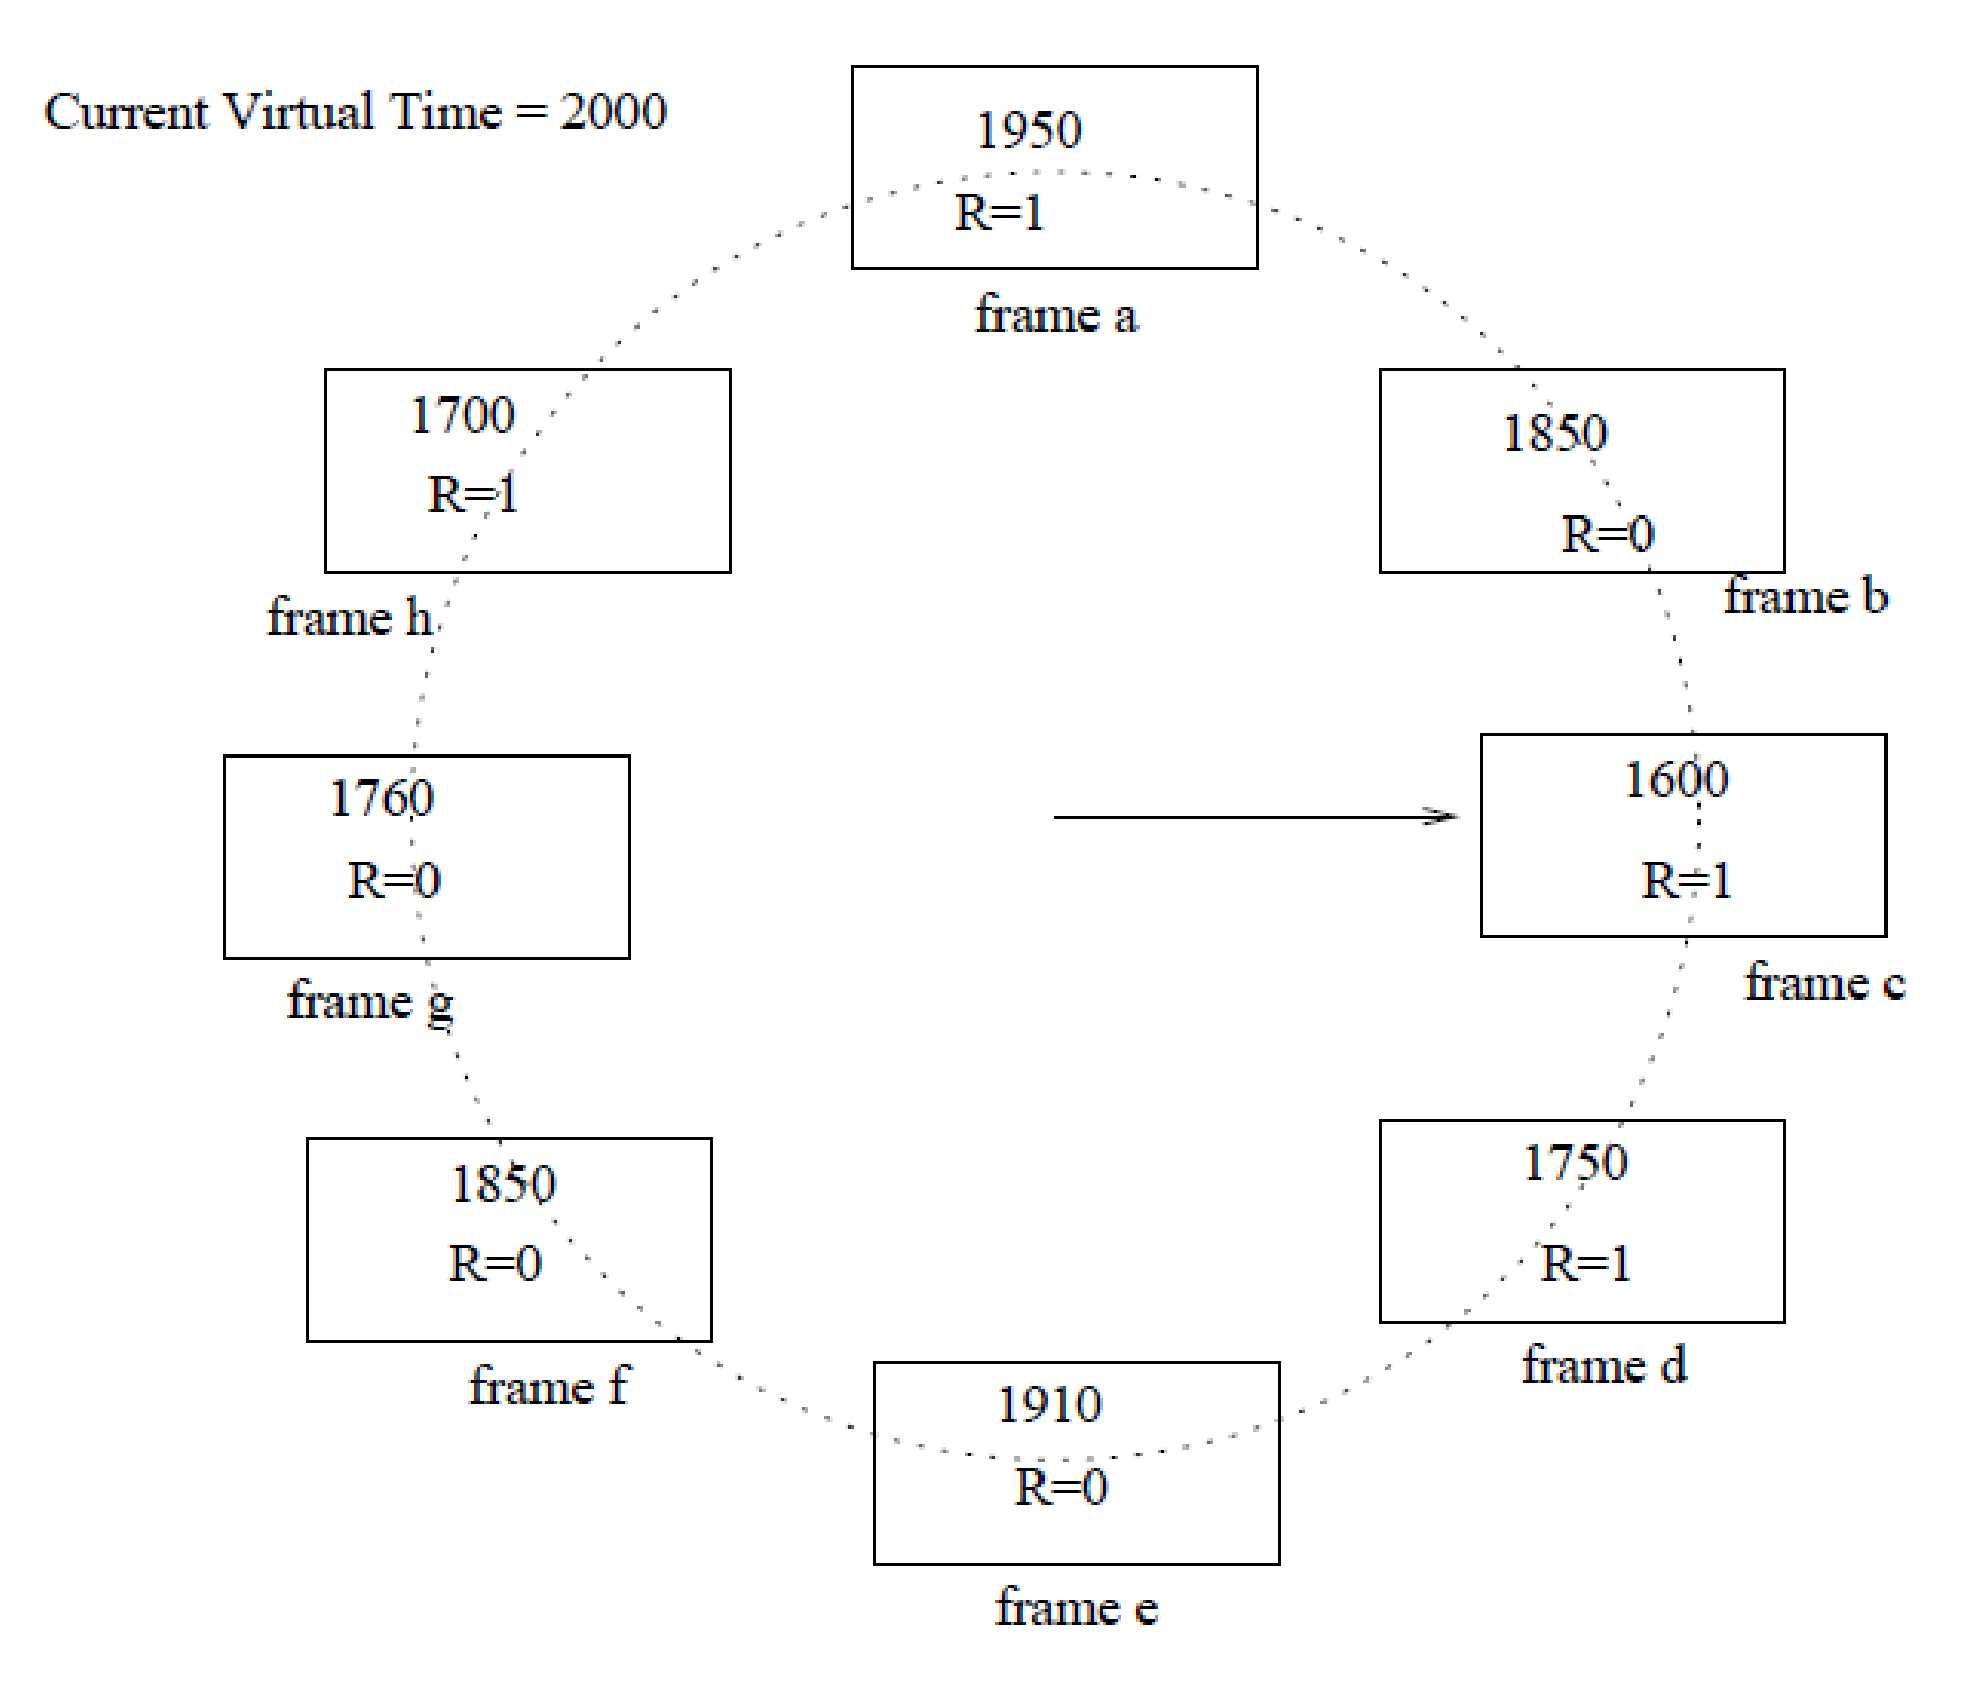
\includegraphics[width=0.75\textwidth]{5.png}
    \end{center}
    \begin{enumerate}
      \item Suppose that the periodic clock interrupt comes virtual time 2000.  Show the new contents of all the frame-list records.
      \item Now suppose that instead of the clock interrupt a page-fault occurs at virtual time 2000.  For each of the two values of \(\tau\) \textbf{equal to 100 and 200}:
        \begin{enumerate}
          \item Indicate the frame whose page is replaced.
          \item Show the new contents of the frame-list.
          \item Determine which logical pages (and thus the corresponding frames storing those pages) will be candidates for removal from the working set.
        \end{enumerate}
    \end{enumerate}
    
  \newpage
  \item Suppose that the page-reference string of a process contains repetitions of long sequences of page references in the range 0 through 511, followed occasionally by a random reference to a page number in the range 512 to 1023.  For example, the sequence: \(0, 1, \hdots, 510, 511, 600, 0, 1, \hdots, 510, 511, 700, 0, 1, \hdots\) consists of the repetitions of the sequence \(0, 1, \hdots, 510, 511\) followed by a random reference to pages such as 600 and 700. Assume that this sequence repeats \(N\) times.
    \begin{enumerate}
      \item If 511 frames are given to this process, how many page-faults would occur using the LRU replacement policy when this sequence repeats for N times?  Answer the this question for the FIFO replacement policy.

      \item With 511 frames allocated to this process, describe a page replacement scheme that would perform much better than LRU or FIFO.  Give the number of page-faults for your proposed replacement scheme when this sequence repeats for N times?  You may assume that the replacement scheme has knowledge of the access pattern in the page reference string, as described above.
    \end{enumerate}

  \newpage
  \item Please read Chapters 1 and 2 from the book O’Reilly book ``Linux Device Drivers'', and answer the following question: \\
    What is the purpose of the following kernel functions?
    \begin{enumerate}
      \item insmod
      \item lsmod
      \item module\_init
      \item module\_exit
    \end{enumerate}
\end{enumerate}
\end{document}
